\chapter{Domain Names, SSL, and Versioning\\
\medium{\textit{---Version 1.0.0}}}
\ChapterLabel{Domain Names, SSL, and Versioning}
\index{Chapter!Domain Names, SSL, and Versioning}

\section{Domain Name}
The following is the name of our Overleaf Domain:
\href{https://mgboverleaf.me}{mgboverleaf.me}

\section{Research SSL Options}
Adding SSL or TLS certificates will allow to secure a self-hosted Overleaf instance so that users can connect over HTTPS. Through some reasearch, the easiest method found is to use a rever proxy (something like Nginx) in front of the Overleaf container to handle the SSL. The following is a way we found to add the SSL:

The first thing that we need is to set up a reverse proxy by running Overleaf normally with HTTP on port 3000 and configure Nginx to listen on ports 80 and 443. The proxy will forward secure requests to Overleaf.

After that, we need to get a free SSL certificate. We can use Let's Encrypt to issue a certificate for our domain. These certificates are free but expire every 90 days.

Next, we have to install the certificate. We have to point Nginx to the vertificate and key files, using the path of the files and comman lines such as \texttt{ssl\_certificate} and \texttt{ssl\_certificate\_key}.

Now, we enable the HTTPS by restarting Nginx and visiting our Overleaf site through out domain with the \texttt{https} in the URL.

We can also set up auto renewal that allows Let's Encrypt to renew certificates every three months through the following command:

\begin{minted}[breaklines]{bash}
sudo certbot renew --quiet --post-hook "systemctl reload nginx"
\end{minted}

\section{Configure Overleaf Container}
\begin{figure}[H]
  \centering
  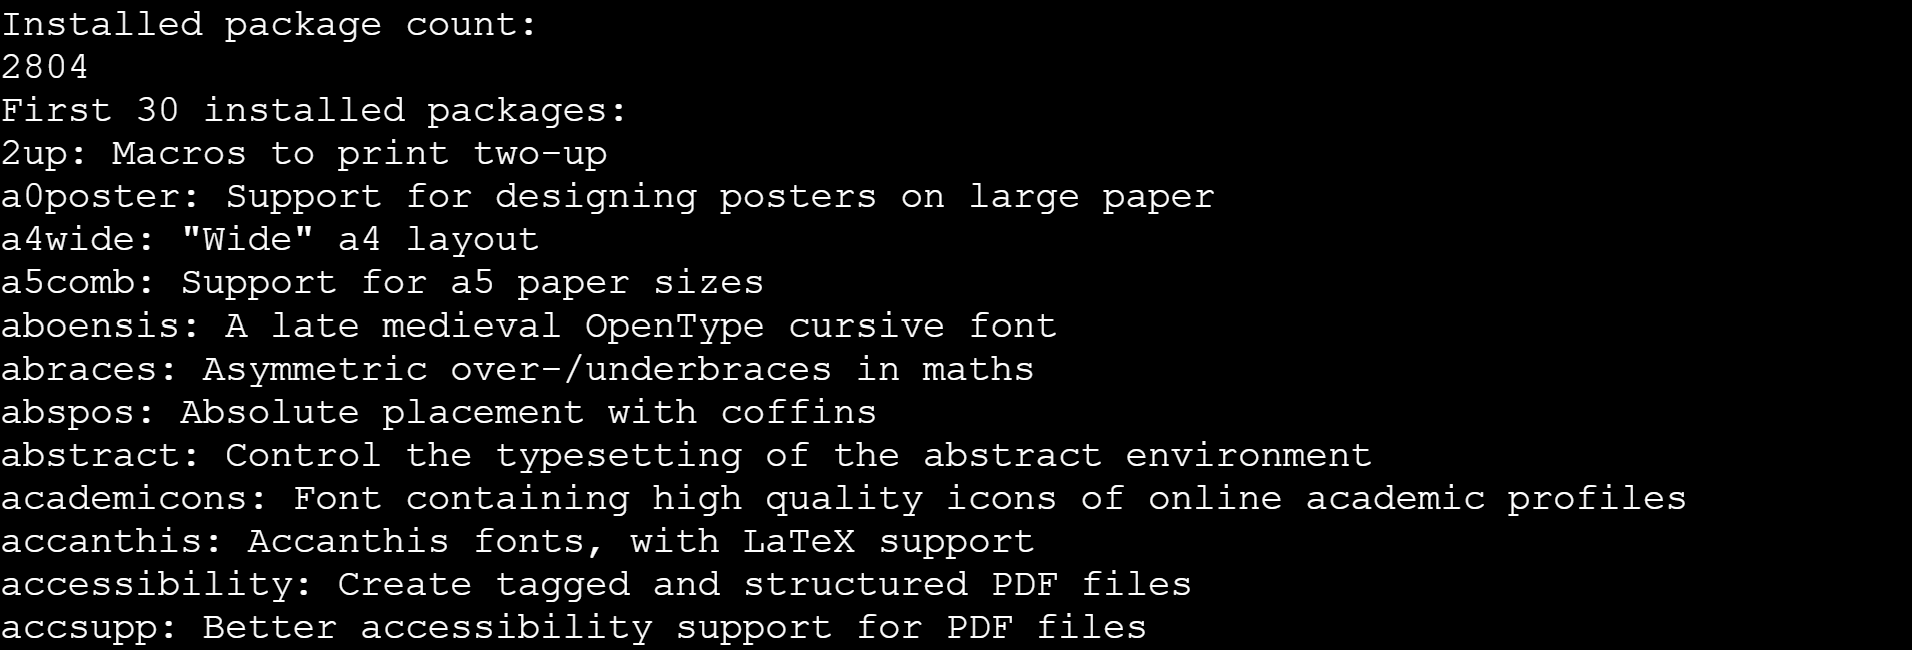
\includegraphics[width=\textwidth]{png/packages.png}
  \caption{LaTeX packages}
  \vspace{-0.3cm}
\end{figure}

\begin{figure}[H]
  \centering
  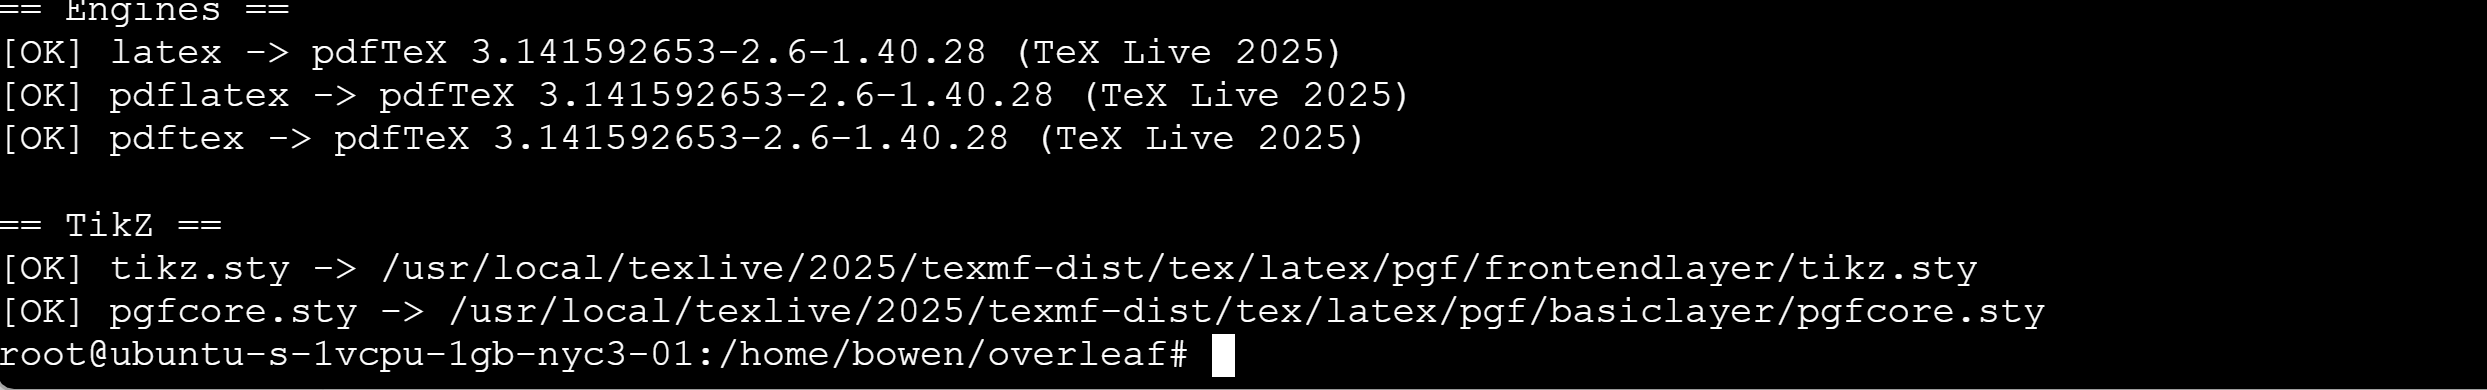
\includegraphics[width=\textwidth]{png/proof.png}
  \caption{Examples for the LaTeX packages}
  \vspace{-0.3cm}
\end{figure}

\begin{figure}[H]
  \centering
  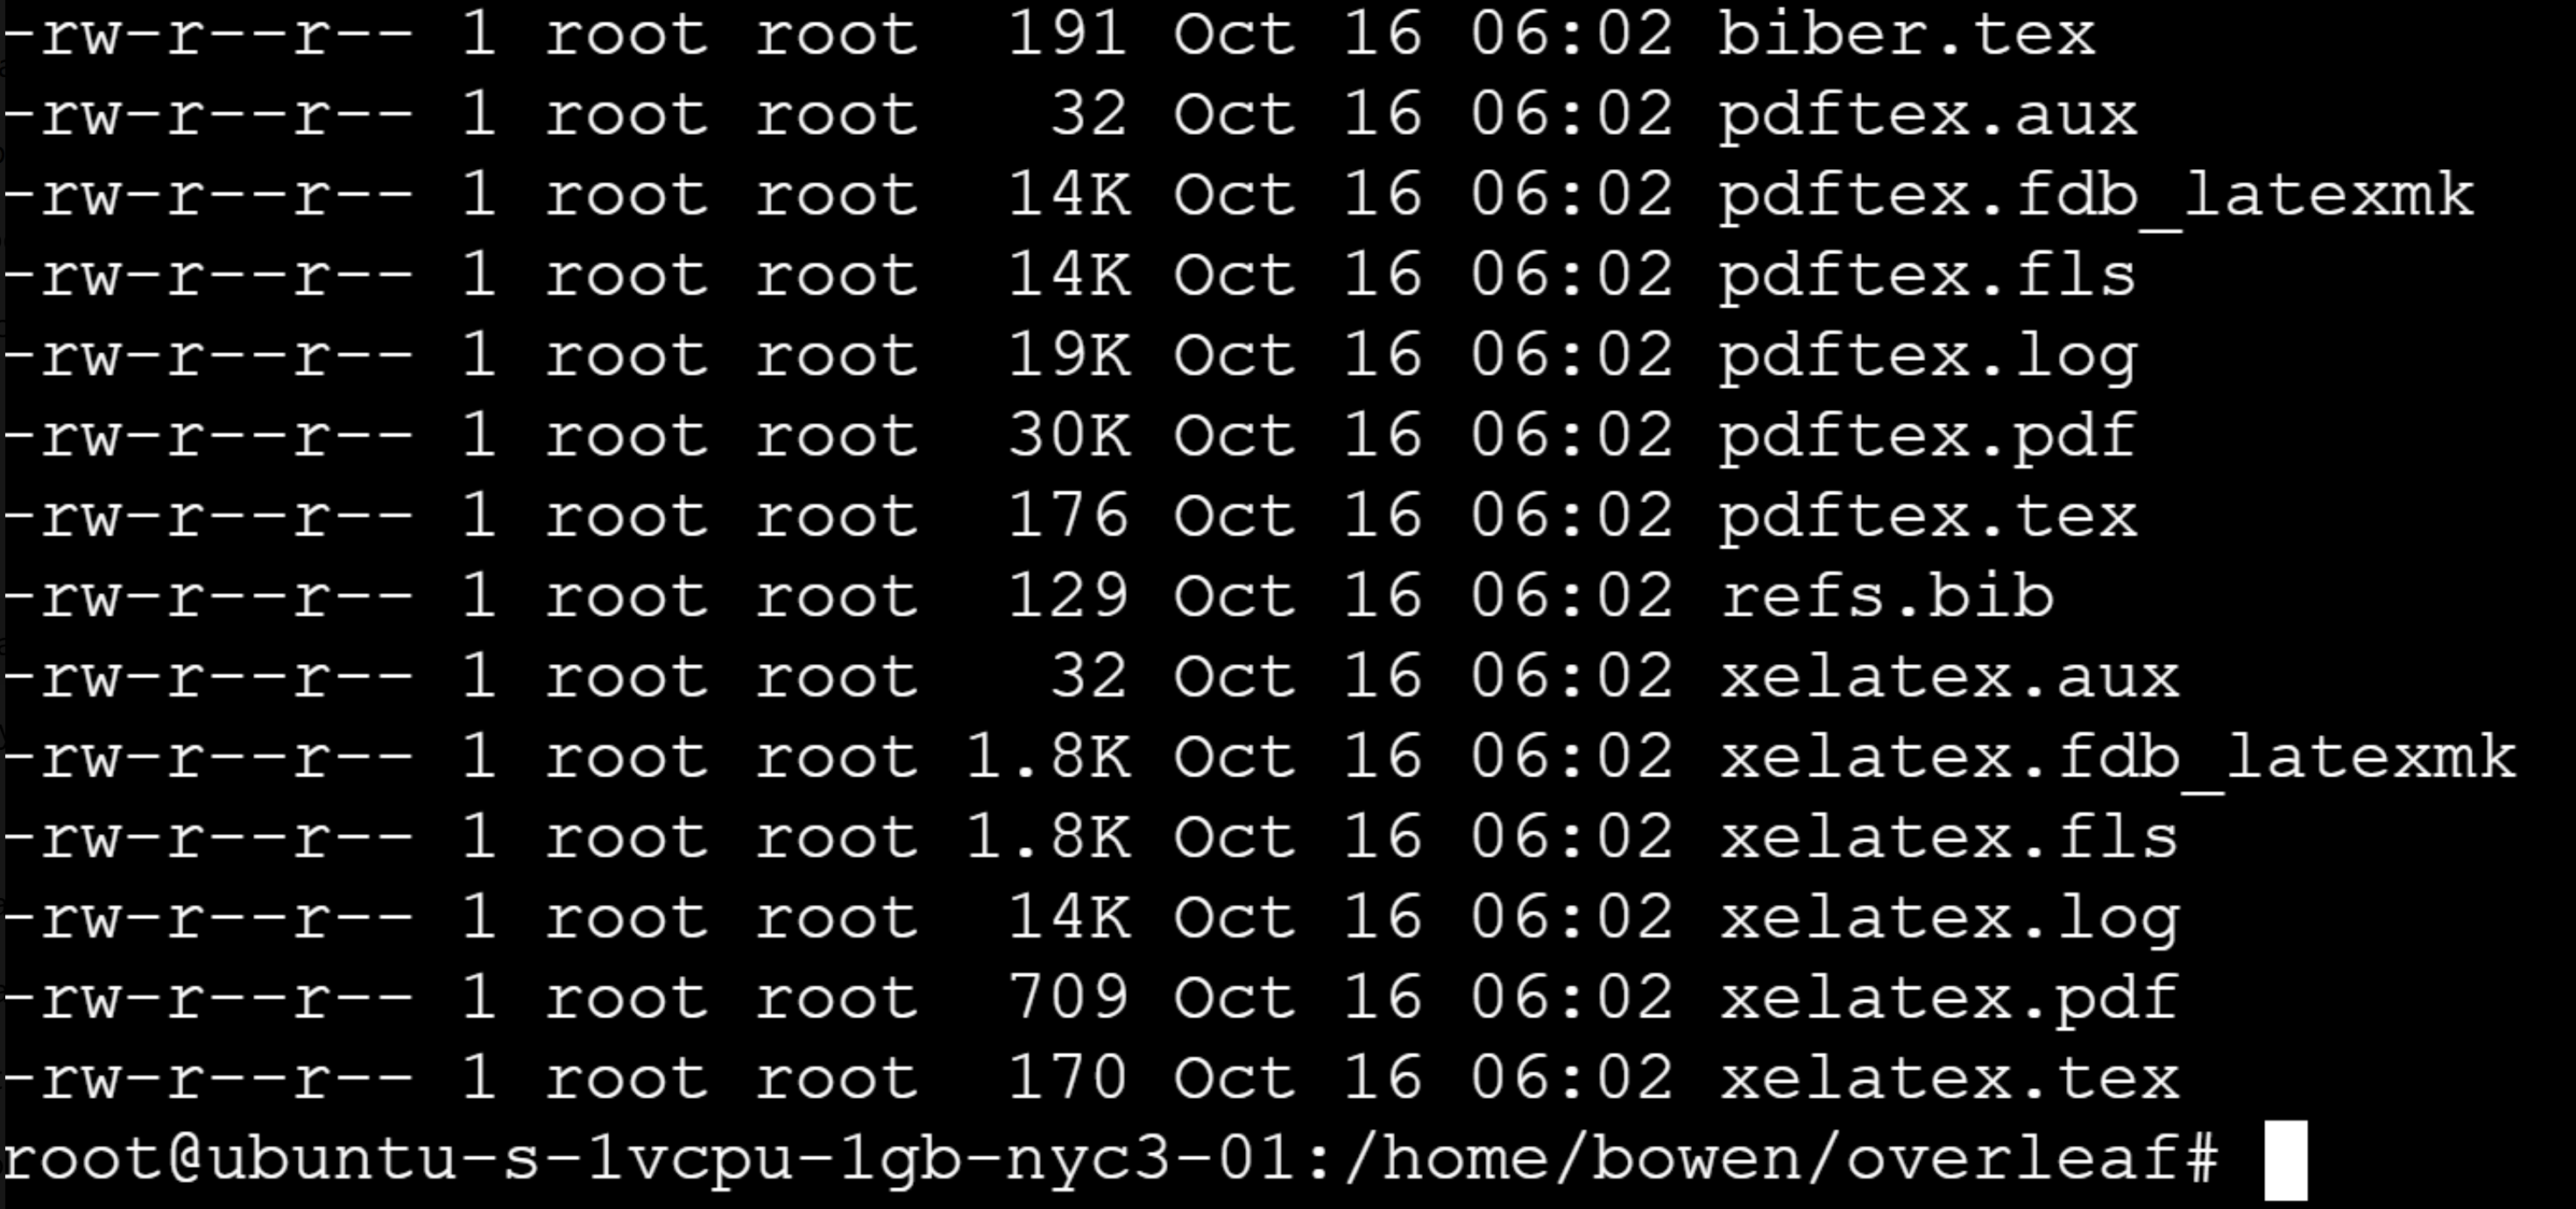
\includegraphics[width=\textwidth]{png/proof2.png}
  \caption{Examples for the LaTeX packages 2}
  \vspace{-0.3cm}
\end{figure}

\begin{itemize}
  \item TeX Live is installed and populated: the output showing 2804 packages had been installed.
  \item Core LaTeX engines are available: version lines for latex, pdflatex, and pdftex demonstrate the compilers are installed.
  \item Bibliography toolchain is present: biber is installed and accessible.
\end{itemize}

\section{Connect Overleaf Instance}
Instructions were created with the help of ChatGPT

GitHub URL: \href{https://github.com/JKDX4567/mgb-overleaf}{https://github.com/JKDX4567/mgb-overleaf}

To connect the Overleaf instance to GitHub, we went with the Git Bridge path. For this to work with our project, we first had to enable the git bridge on our Overleaf server by setting \texttt{GIT\_BRIDGE\_ENABLED=true} in the \texttt{config/overleaf.rc} in our config and then restart Overleaf.

After enabling the git bridge, we open the project that we want to sync, which is this document in our case.

After selecting the project, we have to get its Git URL, which we can do from the Overleaf UI. To do this, we had to go to Menu \textrightarrow{} Git. This will show the Git clone URL: 
\begin{lstlisting}[style=linuxstyle, language=bash]
git clone https://git@git.overleaf.com/68c0867ec3256f4a94db8086
\end{lstlisting}

After getting the Git URL, we have to get the Overleaf Git Token. We need this token so that we can authenticate git for our project. This token is a one time token that we can use to log in to our Overleaf in Git so that we can connect the two.

After getting the token, we can clone the project using the Git link that we created previously. During the cloning process, Git asks for a username and password, which we use our own username for the username and the token as the password.

After this, we are pretty much complete. Now with this setup, we can test syncing our files between Github and Overleaf.

\section{Compile Overleaf}
Instructions were created with the help of ChatGPT

We had two ways that we compiled our Overleaf project. The first method that we used was using \texttt{latexmk} as a command line to automatically run multiple commands at once, bib/biber, and indexing. The following were the lines of code that we used to compile the project:

\begin{lstlisting}[style=linuxstyle, language=bash]
# First, we need to be sure that we are in the correct directory with the use of cd.
cd path/of/directory

# After making sure we are in the correct directory, we use latexmk to put multiple other commands into one simple one.
latexmk -pdf -interaction=nonstopmode -file-line-error --shell-escape itManual.tex
\end{lstlisting}

The other way that we managed to compile our project is directly in Overleaf using its own compiler. The following are the things that we did to get it working correctly using the Menu buttons and its options:

\begin{itemize}[leftmargin=*]
  \item Menu \textrightarrow{} Compiler: \texttt{pdfLaTeX}
  \item Menu \textrightarrow{} Allow shell escape: \texttt{ON} (needed for minted)
  \item Menu \textrightarrow{} Main document: \texttt{itManual.tex}
  \item Click \textbf{Recompile} (or turn on \textbf{Auto})
  \item If ToC/LOF/LOT or links look stale: Menu \textrightarrow{} \textbf{Clear cached files}, then \textbf{Recompile}
\end{itemize}
